 \section{Case Studies}
\label{sec:case_study} 
In Model Based Safety Engineering, the model is developed using a systems engineering language or tool. At this point, a fault model can be developed based on the components of the system under consideration. In order to demonstrate the fault modeling capabilities of the Safety Annex in Section~\ref{sec:fault_modeling}, this section sets the foundation by describing a system with a variety of complex subcomponents. 

\begin{figure}[h!]
	\centering
	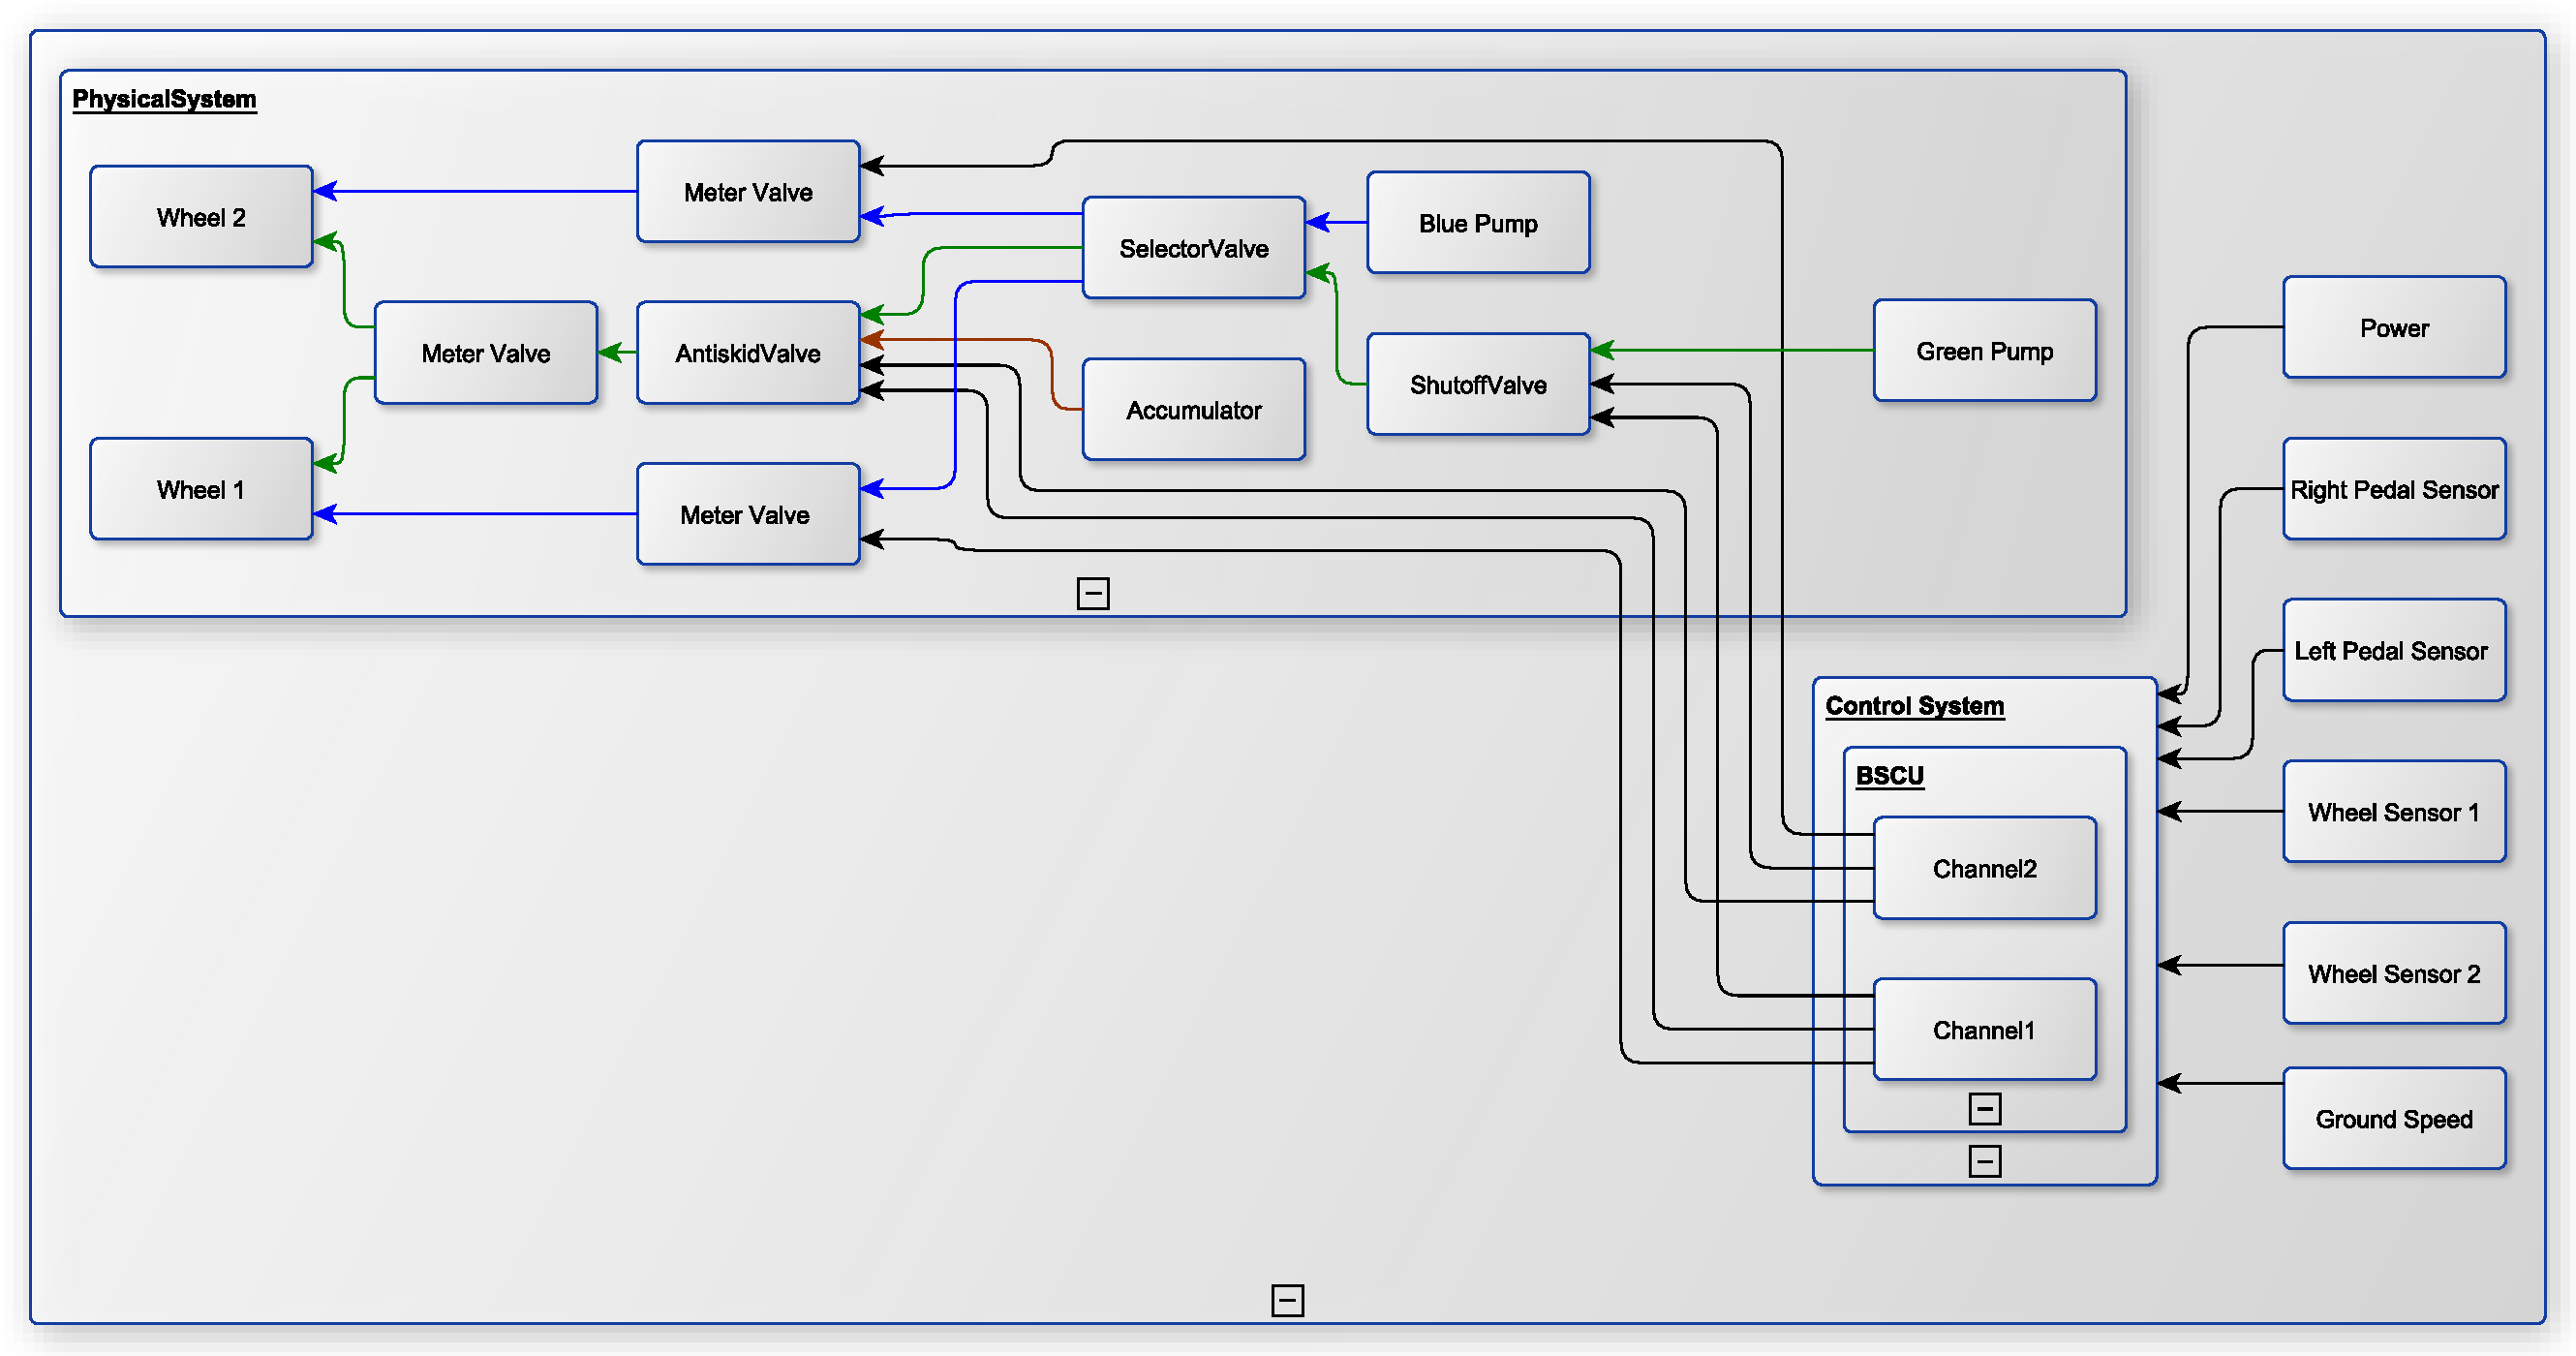
\includegraphics[trim=0 9 0 5,clip,width=\textwidth]{images/wbs_arch.pdf}
	\caption{Wheel Brake System}
	\label{fig:wbs}
\end{figure} 

\subsection{Wheel Brake System}
The Wheel Brake System (WBS) described in AIR6110~\cite{AIR6110} is a well-known example that has been used as a case study for safety analysis, formal verification, and contract based design~\cite{DBLP:conf/cav/BozzanoCPJKPRT15, 10.1007/978-3-319-11936-6-7, CAV2015:BoCiGrMa, Joshi05:SafeComp}. The preliminary work for the safety annex used a simplified model of the WBS~\cite{Stewart17:IMBSA}. In order to demonstrate a complex fault modeling process, we constructed a functionally and structurally equivalent AADL version of one of the most complex WBS NuSMV/xSAP models (arch4wbs) described in~\cite{DBLP:conf/cav/BozzanoCPJKPRT15}. We refer readers to this publication for diagrams of the arch4wbs model~\cite{DBLP:conf/cav/BozzanoCPJKPRT15}.   

\subsubsection{WBS architecture description}
The WBS is composed of two main parts: the control system and the physical system. The control system electronically controls the physical system and contains a redundant Braking System Control Unit (BSCU) in case of failure. The physical system consists of the hydraulic circuits running from hydraulic pumps to wheel brakes. This is what provides braking force to each of the 8 wheels of the aircraft.

There are three operating modes in the WBS model. In \textit{normal} mode, the system uses the \textit{green} hydraulic circuit. The normal system is composed of the green hydraulic pump and one meter valve per each of the 8 wheels. Each of the 8 meter valves are controlled through electronic commands coming from the BSCU. These signals provide brake commands as well as antiskid commands for each of the wheels. The braking command is determined through a sensor on the pilot pedal position. The antiskid command is calculated based on information regarding ground speed, wheel rolling status, and braking commands.

In \textit{alternate} mode, the system uses the \textit{blue} hydraulic circuit.  The wheels are all mechanically braked in pairs (one pair per landing gear). The alternate system is composed of the blue hydraulic pump, four meter valves, and four antiskid shutoff valves. The meter valves are mechanically commanded through the pilot pedal corresponding to each landing gear. If the system detects lack of pressure in the green circuit, the selector valve switches to the blue circuit. This can occur if there is a lack of pressure from the green hydraulic pump, if the green hydraulic pump circuit fails, or if pressure is cut off by a shutoff valve. If the BSCU channel becomes invalid, the shutoff valve is closed.

The last mode of operation of the WBS is the \textit{emergency} mode. This is supported by the blue circuit but operates if the blue hydraulic pump fails. The accumulator pump has a reserve of pressurized hydraulic fluid and will supply this to the blue circuit in emergency mode.

The model contains 30 different kinds of components, 169 component instances, a model depth of 5 hierarchical levels.  The model includes one top-level assumption and  11 top-level system properties, with 113 guarantees allocated to subsystems.  There are a total of 33 different fault types and 141 fault instances within the model.  The large number of fault instances is due to the redundancy in the system design and its replication to control 8 wheels. 

An example property is to ensure no inadvertent braking of each of the 8 wheels.  This means that if all power and hydraulic pressure is supplied (i.e., braking is commanded), then either the aircraft is stopped (ground speed is zero), or the mechanical pedal is pressed, or brake force is zero, or the wheel is not rolling.













